\documentclass[12pt]{article}
\usepackage{preamble}

\pagestyle{fancy}
\fancyhead[LO,LE]{Физические основы компьютерных \\ и сетевых технологий}
\fancyhead[RO,RE]{Лекции Музыченко Я. Б.}

\fancyfoot[L]{\scriptsize исходники найдутся тут: \\ \url{https://github.com/pelmesh619/itmo_conspects} \Cat}

\renewcommand{\thesection}{}

\begin{document}

    \tableofcontents
    \clearpage

    % begin physics1_2024_09_02.tex

    \section{0. Вводная лекция}

    Задается вопрос: зачем обучающимся программистам нужна физика в учебном плане?

    Приводятся цитаты Л. Богуславского, одного из крупнейших IT инвесторов, и Б. Страуструпа, которые считают,
    что такие фундаментальные дисциплины, как математика, физика, иностранный язык, способствуют развитию
    мышления человека

    Такие компании, как Bell Labs и IBM создали прорывные изобретения в области физики, на основе которых
    построены компьютерные технологии

    В 3-ем семестре курс физики будет состоять из классической механики и основ электричества

    В 4-ом семестре будут темы магнетизма, колебаний, волн и волновых процессов

    В 5-ом семестре будут рассматриваться оптика, основы квантовой физики и квантовые вычисления

    Занятия состоят из лекций, практических и лабораторных занятий.
    Всего в 3-ем семестре будут 5 лабораторных работ


    \section{1. Современная физическая картина мира. Кинематика материальной точки}

        \begin{tcolorbox}[colframe=blue!25, colback=blue!10, title=\textbf{План лекции}]

        \footnotesize
        \begin{itemize}
            \item Историческая справка
            \item Методы и модели в физике
            \item Изучаемые объекты
            \item Физика и другие науки
            \item Фундаментальные взаимодействия
            \item Кинематика материальной точки. Начало
        \end{itemize}
    \end{tcolorbox}



    \textbf{Физика} - раздел естествознания, изучающий свойства и формы движения материи.
    Под материей понимают вещество и поля.

    Научный метод: сначала проводятся наблюдения и эксперименты, из которых выдвигается гипотеза и ищется
    адекватная математическая модель, эта гипотеза проверяется, и если она подтверждается,
    то формируется \textit{теория}

    Пример - открытие Нептуна: в 1781-1845 годах наблюдались аномалии в движении Урана, в 1845 проведение расчетов
    координат новой планеты, а в 1846 обнаружилась новая планета

    Принцип соответствия (Н. Бор, 1923 г.) - каждая новая теория должна включать предыдущую как частный случай

    Изучаемые объекты: вселенная, галактики, звездные системы и планеты, экосистемы, макротела, молекулы, атомы, ядра,
    элементарные частицы

    Всего в физике существуют 4 фундаментальных взаимодействия:

    \begin{tabular}{c|c|c}
        Взаимодействие   & Квант поля & Область взаимодействия                        \\ \hline
        Гравитационное   & гравитон   & масса                                         \\
        Электромагнитное & фотон      & все заряженные частицы, атомы, электротехника \\
        Слабое           & бозон      & радиоактивный распад                          \\
        Сильное          & глюон      & атомные ядра, фундаментальные частицы         \\
    \end{tabular}

    Механика - раздел физики, изучающий механическое движение, то есть движение тел в пространстве и времени.
    Механическое движение тел ОТНОСИТЕЛЬНО.

    \begin{tabular}{c|c|c|}
        & $\ll 3 \cdot 10^8$ м/с & $\approx 3 \cdot 10^8$ м/с \\ \hline
        $\gg 1$ нм & Классическая           & Релятивистская             \\ \hline
        $\ll 1$ нм & Квантовая              & Квантовая теория поля      \\ \hline
    \end{tabular}

    Материальная точка - тело, размерами которого можно пренебречь в условиях данной задачи

    Абсолютно твердое тело (АТТ) - система материальных точек, расстояние между которыми не меняется
    в процессе движения (деформации в процессе движения пренебрежимо малы)

    Тело отсчета - тело, относительно которого определяется положение других тел в пространстве

    Система отсчета - совокупность тела отсчета, связанной с ним системы координат и синхронизированных между собой часов

    % векторный, координатный и естественный способы

    Степени свободы - число независимых скалярных величин, однозначно определяющих положение тела в пространстве

    Материальная точка: $3$ степени свободы

    Система N материальных точек: $3N$ степени свободы

    АТТ: $6$ степеней свободы

    Система единиц (\deutscht{le System International d'unites}), 1960

    $[t] = $ с \quad $[S, l] = $ м

    7 основных единиц:

    $[S] = $ м \quad $[T] = $ К

    $[m] = $ кг \quad $[\nu] = $ моль

    $[t] = $ с \quad $[l] = $ Кд

    $[q] = $ Кл

    Изначально все физические единицы основывались на материальных предметов, из-за которых точности единиц была низкой,
    но недавно все единицы были переопределены на основе физических констант.

    В природе нет абсолютно точных вычислений. Измерение любой физической величины без погрешности не имеет смысла!
% end physics1_2024_09_02.tex

% begin physics1_2024_09_09.tex

    \section{2. Кинематика материальной точки}

    \begin{tcolorbox}[colframe=blue!25, colback=blue!10, title=\textbf{План лекции}]

        \footnotesize
        \begin{itemize}
            \item Основные способы описания движения

            \item Основные понятия кинематики

            \item Кинематика поступательного и вращательного движения

            \item Прямая и обратная задачи кинематики

            \item Численные методы при решении задач
        \end{itemize}
    \end{tcolorbox}

    \Def Кинематика - раздел механики, изучающий движение тел, независимо от причин, вызывающих это движение.

    \Def Траектория - линия, по которой движется материальная точка в пространстве

    \Def Путь - длина траектории

    \Def Перемещение - вектор, проведенный из начальной точки в конечную

    \smallvspace

    \textbf{Способы описания движения}

    \begin{multicols}{3}

        \begin{tcolorbox}
            Векторный способ
        \end{tcolorbox}

        \begin{tcolorbox}
            Координатный способ
        \end{tcolorbox}

        \begin{tcolorbox}
            Естественный (траекторный) способ
        \end{tcolorbox}

    \end{multicols}

    \begin{multicols}{3}

        Положение точки может быть однозначно определено с помощью радиус-вектора

        \smallvspace

        Положение точки может быть однозначно определено с помощью трех скалярных координат

        Положение точки определяется дуговой координатой

        \phantom{.}

    \end{multicols}

    \textbf{Векторный способ}

    $\vec{r_1}, \vec{r_2}$ - радиус-векторы, определяющие положения материальной точки в 1 и 2

    $\Delta \vec{r} = \vec{r_2} - \vec{r_1}$ - перемещение материальной точки

    \Def Скорость - векторная физическая величина, характеризующая быстроту перемещения материальной точки

    Средняя скорость - $\Pair{\vec{v}} = \frac{\Delta \vec{r}}{\Delta t}$

    Мгновенная скорость - $\vec{v} = \lim_{\Delta t \to 0} \frac{\Delta \vec{r}}{\Delta t} = \frac{d \vec{r}}{dt}$

    Средняя путевая скорость - $v_{\text{ср}} = \frac{\Delta S}{\Delta t}$

    \Def Ускорение - векторная физическая величина, характеризующая быстроту изменения скорости материальной точки

    Среднее ускорение - $\Pair{\vec{a}} = \frac{\Delta \vec{v}}{\Delta t}$

    Мгновенное ускорение - $\vec{a} = \lim_{\Delta t \to 0} \frac{\Delta \vec{v}}{\Delta t} = \frac{d \vec{v}}{dt}$

    % годограф скорости

    \textbf{Координатный способ}

    В координатном способе положение точки описано 3 координатами $x, y, z$ (в данном случае в ДПСК)

    $|r| = \sqrt{x^2 + y^2 + z^2}$

    $\vec{r} (t) = r_x (t) \vec{\imath} + r_y (t) \vec{\jmath} + r_z (t) \vec{k} = x(t) \vec{\imath} + y(t) \vec{\jmath} + z(t) \vec{k}$

    $\vec{v} (t) = \frac{d \vec{r}}{dt} = \frac{dx}{dt} \vec{\imath} + \frac{dy}{dt} \vec{\jmath} + \frac{dz}{dt} \vec{k}$

    $\vec{v} (t) = v_x(t)\vec{\imath} + v_y(t) \vec{\jmath} + v_z(t) \vec{k}$

    $|\vec{v}| = \sqrt{v_x^2 + v_y^2 + v_z^2}$


    % ускорение

    Прямая задача:

    $\vec{r}(t), x(t), y(t), z(t) \longrightarrow \vec{v}(t), \vec{a}(t), v_x, v_y, v_z, a_x, a_y, a_z$

    Решением является дифференцирование

    Обратная задача:

    $\vec{a}(t), a_x, a_y, a_z \longrightarrow \vec{v}(t), \vec{r}(t), x(t), y(t), z(t)$

    Для обратной задачи решением является интегрирование

    $\vec{v} = \frac{d\vec{r}}{dt} \quad d\vec{r} = \vec{v}dt \quad \Delta\vec{r} = \int_{t_1}^{t_2} \vec{v}dt$

    \begin{tcolorbox}
        $\vec{r} = \vec{r_0} + \Delta \vec{r} = \vec{r_0} + \int_{t_1}^{t_2} \vec{v}dt$
    \end{tcolorbox}

    Аналогично для ускорения

    Численное решение ОДУ (обыкновенного дифференциального уравнения) $\frac{dy}{dx} = f(x, y)$ на отрезке $[x_0, x_n]$ при условии $y(x_0) = y_0$

    Разбиваем отрезок $[x_0, x_n]$ на конечное число частей введением узловых точек

    Шаг разбиения: $h = \frac{x_N - x_0}{N}$

    По определению производной $\frac{dy}{dx} = \frac{y_{i + 1} - y_i}{h}$, из этого:

    \begin{tcolorbox}
        Формула Эйлера: $y_{i + 1} = y_i + hf(x_i, y_i)$
    \end{tcolorbox}

    $dy = f(x, y) dx$

    $\Delta y = y_{i + 1} - y_i = \int_{x_i}^{x_{i + 1}} f(x, y) dx$

    \textbf{Естественный (траекторный) способ}

    Если траектория точки заранее известна, то положение точки задается дуговой координатой $l(t)$

    $\vec{v} = v_\tau \vec{\tau} \quad v_\tau \frac{dl}{dt} |\vec{\tau}| = 1$

    $\vec{a} = \frac{d\vec{v}}{dt} = \frac{dv_\tau}{dt} \vec{\tau} + \frac{d\vec{\tau}}{dt} v_\tau \quad\quad\quad \frac{d\tau}{dt} = \frac{d\tau}{dl} \cdot \frac{dl}{dt} = \frac{d\tau}{dl} v_\tau$

    $\vec{a} = \frac{d\vec{v}}{dt} = \frac{dv_\tau}{dt} \vec{\tau} + \frac{d\vec{\tau}}{dt} v_\tau^2 $

    $d\tau = \tau d\alpha$

    $dl = R d\alpha \quad\quad\quad d\vec{\tau} \uparrow\uparrow \vec{n}$

    $R$ - радиус кривизны траектории

    $\vec{\alpha} = \frac{dv_\tau}{dt} \vec{\tau} + \frac{1}{R} v_\tau^2 \vec{n} \quad\quad\quad \vec{a} = \vec{a_\tau} + \vec{a_n}$

    Тангенциальное ускорение отвечает за изменение модуля скорости, направлено по касательной к траектории движения

    Нормальное ускорение отвечает за изменение направления вектора скорости, направлено к центру кривизны траектории
% end physics1_2024_09_09.tex

% begin physics1_2024_09_16.tex

    \section{3.
    Кинематика вращательного движения.
    Динамика материальной точки}

    \begin{tcolorbox}[colframe=blue!25, colback=blue!10, title=\textbf{План лекции}]

        \footnotesize
        \begin{itemize}
            \item Угловые величины: угол поворота, угловая скорость

            \item Взаимосвязь между линейными и угловыми величинами

            \item Плоское движение

            \item Динамика материальной точки

            \item Законы Ньютона. Силы в механике

            \item Принципы работы акселерометра
        \end{itemize}
    \end{tcolorbox}

    \subsection{Движение по окружности}

    Возьмем точку $A$, положение которое определим через $\vec{r}$. Точка $A$ движется по окружности вокруг неподвижной оси $OO^\prime$

    Тогда $d\vec{r}$ - перемещение, $d\vec{\varphi}$ - элементарный угол поворота (вектор определяет в какую сторону, по часовой или против,
    обращается по окружности тело; вектор направлен перпендикулярно окружности)

    $|d\vec{r}| = Rd\varphi = r \cdot \sin \alpha d \varphi$

    $R = r \cdot \sin \alpha$

    $d\vec{r} = [d \vec{\varphi} \vec{r}]$ \hfill {\scriptsize здесь и далее $[\vec{x}\vec{y}]$ - векторное произведение}

    Угловая скорость - векторная величина, показывающая как меняется угол поворота тела со временем: $\Pair{\omega} = \frac{\Delta \varphi}{\Delta t} \quad\quad\quad \vec{\omega} = \frac{d\vec{\varphi}}{dt}$

    Направление совпадает с направлением угла поворота $d\vec{\varphi}$: $\vec{\omega} \uparrow\uparrow d\vec{\varphi}$

    Угловое ускорение - векторная величина, показывающая как меняется угловая скорость тела со временем

    $\Pair{\beta} = \frac{\Delta \omega}{\Delta t} \quad\quad \vec{\beta} = \frac{d\vec{\omega}}{dt} = \frac{d^2 \vec{\varphi}}{dt^2}$

    Направление совпадает с направлением вектора изменения скорости $\Delta \vec{\omega}$: $\vec{\beta} \uparrow\uparrow d\vec{\omega}$

    $d\vec{r} = [d\vec{\varphi} \vec{r}]$

    $dr = d\varphi \cdot r \cdot \sin \alpha = d\varphi \cdot R$

    Выразим скорость $\vec{v} = \frac{d\vec{r}}{dt} = [\frac{d\vec{\varphi}}{dt}\vec{r}] = [\vec{\omega} \vec{r}]$

    $v = \omega \cdot r \cdot \sin \alpha = \omega \cdot R$

    Выразим ускорение: $\vec{a} = \frac{d\vec{v}}{dt} = [\frac{d\vec{\omega}}{dt} \vec{r}] + [\vec{\omega} \frac{d\vec{r}}{dt}] = [\vec{\beta}\vec{r}] + [\vec{\omega}\vec{v}] = \vec{a}_\tau + \vec{a}_n$

    $\vec{a}_\tau$ называют тангенциальным ускорением (напраленным по касательной), $\vec{a}_n$ - нормальным (направленным к центру)

    $a_\tau = \beta \cdot r \cdot \sin\alpha = \beta \cdot R$

    Перемещение, путь, скорость:

    \begin{multicols}{2}

        $d\vec{r} = [d\vec{\varphi} \vec{\rho}] (\vec{\rho}\text{ - вектор радиуса окружности})$

        $dr = d\varphi \cdot R$

        $S = \varphi \cdot R$

        $\vec{v} = [\vec{\omega} \vec{\rho}]$

        $v = \omega \cdot R$

    \end{multicols}

    Ускорение: $\vec{a} = [\vec{\beta}\vec{r}] + [\vec{\omega}\vec{v}]$

    \begin{multicols}{3}

        $\vec{a}_\tau = [\vec{\beta}\vec{r}]$

        $a_\tau = \beta \cdot R$

        $\vec{a}_n = [\vec{\omega}\vec{v}] = [\vec{\omega}[\vec{\omega}\vec{\rho}]]$

        $a_n = \omega^2 R = \frac{1}{R} v^2$

        $T = \frac{2\pi}{\omega} = \frac{1}{\nu}$ - период

        $\nu = \frac{\omega}{2\pi} = \frac{1}{T}$ - частота

    \end{multicols}

    Плоское движение - движение твердого тела, при котором каждая его точка движется в плоскости,
    параллельной некоторой неподвижной в данной системе отсчета плоскости

    $\vec{r} = \vec{r}_0 + \vec{r}^\prime$

    $d\vec{r} = d\vec{r}_0 + d\vec{r}^\prime = d\vec{r}_0 + [d\vec{\varphi}\vec{r}]$

    $\vec{v} = \vec{v}_0 + [\vec{\omega}\vec{r}]$

    $\vec{v}_C$ - скорость центра колеса относительно точки отсчета

    $\vec{v}_{\text{вр}}$ - скорость точек колеса относительное его центра

    \Def Динамика - раздел механики, изучающий причины, вызывающие движение тел

    1687 г. - законы Ньютона, основа классической механики (механики Ньютона), обобщение большего количества опытов (Г. Галилей)

    Классическая механика - частный случай  1) СТО при скоростях много меньших скорости света $v \ll c$;
    2) квантовой механики при массах, много больших массы атома

    В динамике существуют различия между системами отсчета и преимущества одних СО над другими.

    Существуют такие системы отсчета, относительно которых свободное тело (тело, на которое не действуют другие тела) движется равномерно
    и прямолинейно или находится в состоянии покоя. Таким системы называются инерциальными (ИСО)

%    Земля $a_n = 3.4 \frac{\text{см}}{\text{с}^2}$
%
%    Центр Земли $a_n = 0.6 \frac{\text{см}}{\text{с}^2}$
%
%    Земля $a_n = 3 \cdot 10^{-8} \frac{\text{см}}{\text{с}^2}$
    % for later use i think

    \mediumvspace

    \textbf{Принцип относительности Галилея:}

    Любая СО, движущаяся с постоянной скоростью относительно ИСО, также является ИСО. Тогда справедливо любое из этих утверждений:

    \begin{enumerate}
        \item все ИСО эквивалентны друг другу по своим механическим свойствам
        \item во всех ИСО свойства пространства и времени одинаковы
        \item законы механики одинаковы во всех ИСО
    \end{enumerate}

    % сложное движение земли
    % перечитываю это и не понимаю, че было

    Преобразования Галилея - преобразования координат при переходе от одной ИСО к другой

    $K, K^\prime$ - ИСО

    $\vec{V}$ - скорость, с которой движется СО $K^\prime$ относительно $K$
    $t = t^\prime$

    $\vec{r} = \vec{r}^\prime + \vec{V}t$

    $\vec{c} = \vec{v}^\prime + \vec{V}$

    $\vec{a} = \vec{a}^\prime$

    \Def Сила - физическая величина, определяющая количественную характеристику и напраление воздействия, оказываемого на данное тело
    со стороны других тел.

    Силы условно можно разделить на силы, возникающие при непосредственном контакте (силы трения, давления) и на силы,
    возникающие через поля (электрические, гравитационные).

    \Def Инертная масса - мера инертности тела, то есть способности тела сохранять свою скорость при движении

    \Def Гравитационная масса - мера гравитацонного взаимодействия, величина, определяющая вес тел.

    $m_{\text{ин}} = m_{\text{гр}}$ с точностью до $10^{-13}$ кг

    В классической механике 1) масса - величина аддитивная ($m_1 + m_2 + \dots = m$); 2) $m = const$


    \subsection{Законы Ньютона}


    \begin{tcolorbox}[colframe=green!25, colback=green!10, title=\textbf{I закон Ньютона}, coltitle=black]
        Существуют такие системы отсчёта, называемые инерциальными, относительно которых материальные точки, когда на них не действуют никакие силы (или действуют силы взаимно уравновешенные), находятся в состоянии покоя или равномерного прямолинейного движения.
    \end{tcolorbox}


    \begin{tcolorbox}[colframe=green!25, colback=green!10, title=\textbf{II закон Ньютона}, coltitle=black]
        Ускорение тела пропорционально действующей на него силе и обратно пропорционально его массе $\vec{a} = \frac{\vec{F}}{m}$
    \end{tcolorbox}

    Под равнодействующей всех сил понимают векторную сумму всех сил, действующих на тело (принцип суперпозиции)

    $\vec{F} = \frac{d\vec{p}}{dt}$ - II закон в импульсной (дифференциальной) форме

    \begin{tcolorbox}[colframe=green!25, colback=green!10, title=\textbf{III закон Ньютона}, coltitle=black]
        Силы, с которыми два тела действуют друг на друга равны по модулю и направлены в противоположные стороны $\vec{F}_{12} = -\vec{F}_{21}$
    \end{tcolorbox}

    Закон Гука: $F = k|\Delta l|$ - сила упругости пропорциональна изменению длины тела

    Акселерометр - прибор, измеряющий ускорение, точнее проекцию кажущегося ускорения.

    Акселерометр использует II закон Ньютона ($mg - k\Delta l = ma$) во всех трех осях, что позволяет
    измерение ускорения в трех направлениях. Акселерометр используется в автомобилях, авиации, телефонах,
    игровых контроллерах, компьютерах (защита жесткого диска). Сейчас акселерометры изготавливаются
    в размерах от 20 мкм до 1 мм из кремния
% end physics1_2024_09_16.tex

% begin physics1_2024_09_30.tex

    \section{4.
    Импульс. Закон сохранения импульса.}

    \begin{tcolorbox}[colframe=blue!25, colback=blue!10, title=\textbf{План лекции}]

        \footnotesize
        \begin{itemize}
            \item Силы в механике

            \item Универсальные законы природы - законы сохранения

            \item Импульс материальной точки

            \item Закон сохранения импульса

            \item Центр масс. Ц-система
        \end{itemize}
    \end{tcolorbox}

    \subsection{Силы в механике. Сила гравитационного взаимодействия}

    Все силы в механике относятся к гравитационным и электромагниным фундаментальным воздействиям.
    Это можно заметить на примере законов всемирного тяготения и Кулона:

    \begin{multicols}{2}
        \begin{center}
            $\vec{F} = G \frac{m_1 m_2}{r^3_{12}} \vec{r}_{12}$

            Закон всемирного тяготения
        \end{center}

        \begin{center}
            $\vec{F} = k \frac{q_1 q_2}{r^3_{12}} \vec{r}_{12}$

            Закон Кулона
        \end{center}
    \end{multicols}

    Запишем закон всемирного тяготения для тела $m$ на расстоянии $r$ от Земли (радиуса $R$ и массы $M_{\text{З}}$):

    \[|\vec{F}| = G\frac{mM_{\text{З}}}{(R + r)^2}\]

    С другой стороны, любое тело вблизи поверхности Земли движется с ускорением свободного падения $\vec{g}$, следовательно,
    сила, действующая на тело, равна:

    \[F = G\frac{mM_{\text{З}}}{R^2} = mg\]

    Одинаково ли ускорение свободного падения на поверхности Земли? % жопа

    \smallvspace

    \begin{minipage}{\textwidth}
        \begin{wrapfigure}{r}{0pt}
            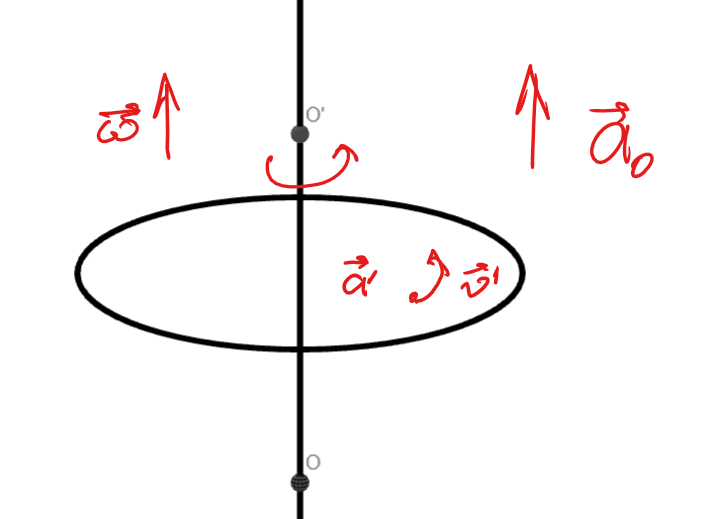
\includegraphics[height=5cm]{physics1/images/physics1_2024_09_30_1}
        \end{wrapfigure}

        Пусть $k$ - ИСО, $k^\prime$ - НИСО (неинерциальная СО), а $\vec{a}^\prime, \vec{v}^\prime$ - ускорение и скорость в системе $k^\prime$,
        а сама система $k^\prime$ движется с ускорением $\vec{a_0}$ и вокруг оси с угловой скоростью $|\vec{\omega}| = const$


        Тогда получаем ускорение в НИСО: $\vec{a}^\prime = \vec{a} + \omega^2 \vec{\rho} + 2 [\vec{v}^\prime \vec{\omega}] - \vec{a}_0$

        $\vec{a}$ - ускорение тела в системе $k^\prime$

        $\omega^2 \vec{\rho}$ - центробежное ускорение

    \end{minipage}

    \smallvspace

    $2 [\vec{v}^\prime \vec{\omega}]$ - ускорение Кориолиса

    $\vec{a}_0$ - поступательное ускорение (системы отсчета $k^\prime$ для $k$)

    $m\vec{a}^\prime = \underset{\sum \vec{F}}{\underbrace{m\vec{a}}} + \underset{\text{силы инерции (т. н. фиктивные)}}{\underbrace{m\omega^2 \vec{\rho} + 2m [\vec{v}^\prime \vec{\omega}] - m\vec{a}_0}}$ - основное уравнение динамики в НИСО

    $m \omega^2 \vec{\rho}$ - центробежная сила

    $2m [\vec{v}^\prime \vec{\omega}]$ - сила Кориолиса

    $m\vec{a}_0$ - поступательная сила инерции


    В НИСО возникают так называемые силы инерции (фиктивные), центробежная и Кориолиса связаны с вращением

    Сила Кориолиса будет действовать только на те тела, которые движутся

    Из закона всемирного тяготения можно вывести ускорение свободного падения гравитационное: $g_{\text{грав}} = G \frac{M_\text{З}}{R^2} = 9.81\dots9.83 \frac{\text{м}}{\text{с}^2}$

    Из этого получить ускорение эффективное: $g_\text{эфф} = g_\text{грав} + a_\text{цб} = 9.78\dots9.83$ (ускорение свободного падения уменьшается на 3 сотых из-за вращения)

    \subsection{Вес тела}

    \Def Вес тела - сила, с которой тело действует на неподвижную относительно него опору

    В случае опоры $|P| = |N|$ ($N$ - сила реакции опоры)

    Рассмотрим случай, когда тело находится в неподвижном состоянии на поверхности:

    $m\vec{g} + \vec{N} = 0 \quad\quad N - mg = 0 \quad\quad P = mg$

    Вес тела равен силе тяжести только при $\vec{a} = 0$ системы отсчета

    \subsection{Силы трения}

    Силы трения появляются при перемещении соприкасающихся тел или их частей относительно друг друга.
    Различают сухое и вязкое трение. К сухому трению относится трение покоя, трение скольжения и трение качения

    \textbf{Сила трения покоя} применима не телам, которые покоятся; она не может превышать некоторого максимального значения: $0 \leq F_\text{тр.} \leq \mu_0 N$ (где $\mu_0$ - коэффициент трения покоя)

    \textbf{Сила трения скольжения} возникает при движении соприкасающихся тел. В общем случае сила трения скольжения зависит
    от скорости движения, но для широкого класса тел равна максимальной силе трения покоя и подчиняется закону Амонтона-Кулона: $F_\text{тр} = \mu N$

    В задачах принимается, что $\mu_0 = \mu$, тогда во время покоя сила трения растет линейно, пока не достигнет $\mu N$, тогда тело начинает движение, и применяется сила трения скольжения

    \subsection{Как можно измерить массу тел?}

    Для измерения массы необходимо сравнить ее с другой, принятой за эталон. Сравним массы $m_1$ и $m_2$

    Опыт показывает, что в замкнутой системе - системе, в которой можно пренебречь взаимодействием с другими телами,
    выполняется соотношение:

    $\frac{\Delta \vec{v}_1}{\Delta \vec{v}_2} = \frac{m_2}{m_1}$

    $\Delta \vec{v}_1 \uparrow \downarrow \Delta \vec{v}_2 \quad\quad\quad v \ll c$

    $m_1 \Delta \vec{v}_1 = -m_2 \Delta \vec{v}_2$ или $m_1 \Delta \vec{v}_1 + m_2 \Delta \vec{v}_2 = 0$

    Импульс (количество движения) - векторная величина, равная произведению массы тела на его скорость: $\vec{p} = m\vec{v} \quad\quad [p] = \text{кг} \cdot \text{м/с}$

    Определение справедливо для материальной точки и для поступательного движения твердого тела

    Импульс системы материальных точек: $\vec{P} = \sum_{i = 1}^N \vec{p}_i$

    Для системы $N$ материальных точек ($\vec{F}_i$ - внешние силы)

    $\frac{d\vec{P}}{dt} = \sum \vec{F}_i \quad\quad\quad \vec{P} = const$

    Закон сохранения импульса - импульс замкнутой системы остается постоянным


    При изменении состояния системы всегда существуют такие величины, которые сохраняются с течением времени. Среди этих величин наиболее важное значение имеют импульс, энергия и момент импульса.

    Эти величины обладают свойством аддитивности – значение величин для системы, состоящей из частей, равно сумме значений для каждой из частей в отдельности.

    Законы сохранения – универсальные законы природы, связаны с фундаментальными свойствами пространства и времени.

    \begin{center}
        Закон сохранения импульса – однородность пространства

        Закон сохранения энергии – однородность времени

        Закон сохранения момента импульса – изотропность пространства
    \end{center}
% end physics1_2024_09_30.tex

% begin physics1_2024_10_07.tex

    \section{5. Вращательное движение. Моменты силы и импульса}

    \begin{minipage}{\textwidth}
        \begin{wrapfigure}{r}{0pt}
            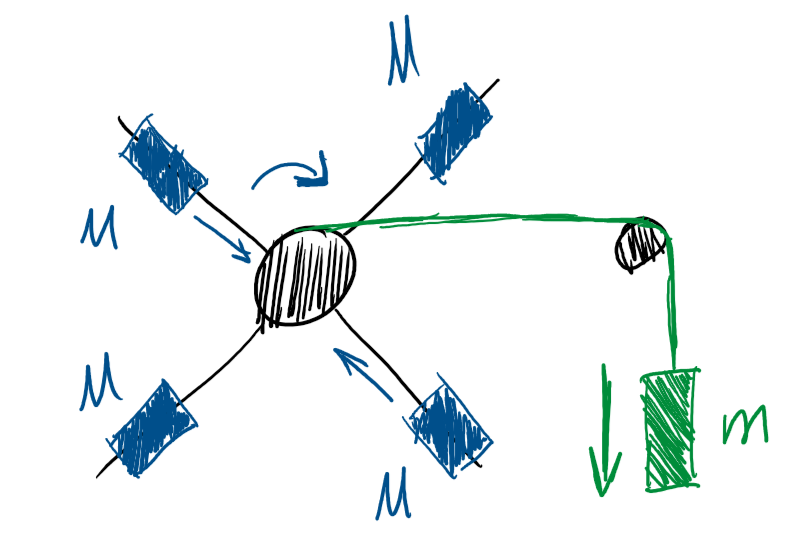
\includegraphics[height=5.5cm]{physics1/images/physics1_2024_10_07_1}
        \end{wrapfigure}

        Одной из лабораторный работ в курсе механики является работа с маятником Обербека (представлен на рисунке).
        Принцип его работы таков: к вращающемуся колесу с грузиками на спицах привязана нить, другой конец которой
        привязан к грузу через блок, груз падает, вращает колесо. В ходе эксперимента можно заметить, что при приближении
        грузиков к центру колесо начинает раскручиваться быстрее.

    \end{minipage}

    \mediumvspace

    Рассмотрим величины, действующие при вращательном движении:

    \smallvspace

    \begin{enumerate}

        \begin{minipage}{\textwidth}
            \begin{wrapfigure}{r}{0pt}
                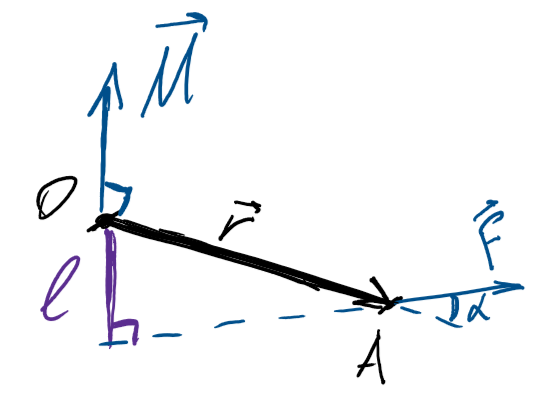
\includegraphics[width=0.3\textwidth]{physics1/images/physics1_2024_10_07_2}
            \end{wrapfigure}

            \item Момент силы $M$

            $M = F \cdot l$

            $\vec{M} = [\vec{r} \vec{F}] \qquad M = r \cdot F \cdot \sin\alpha = l \cdot F$

            Так как момент силы - векторное произведение, то вектор момента силы направлен перпендикулярно к плоскости
            радиус-вектора и вектора силы

            $[M] = \text{Н} \cdot \text{м}$

            % /з

            Аналогично рассмотрим момент силы для противоположных сил:

            \begin{wrapfigure}{r}{0pt}
                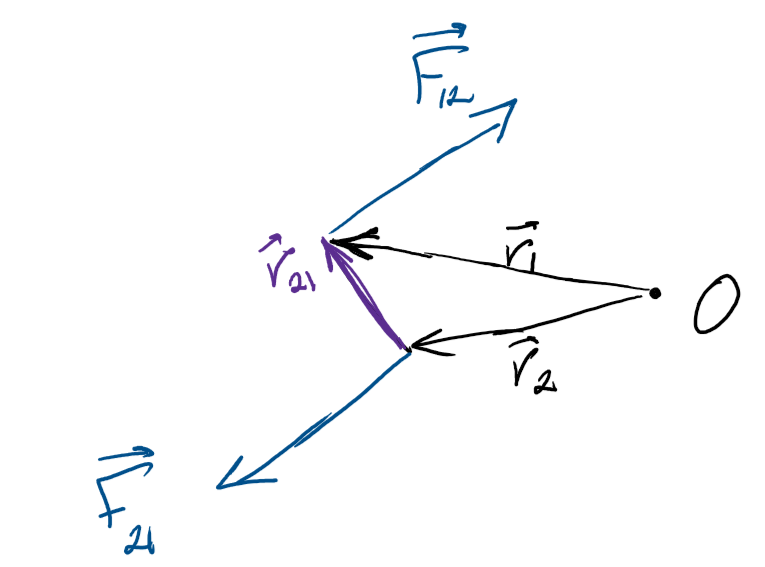
\includegraphics[width=0.3\textwidth]{physics1/images/physics1_2024_10_07_3}
            \end{wrapfigure}

            \item Момент пары сил

            $\vec{M} = \vec{M}_1 + \vec{M}_2 = [\vec{r}_1 \vec{F}_{12}] + [\vec{r}_2 \vec{F}_{21}] =
            [(\vec{r}_2 + \vec{r}_{21}) \vec{F}_{12}] + [\vec{r}_2 \vec{F}_{21}] = [\vec{r}_2 \vec{F}_{12}] + [\vec{r}_{21} \vec{F}_{12}] + [\vec{r}_2 \vec{F}_{21}]$

            $\vec{M} = [\vec{r}_{21} \vec{F}_{12}] = [\vec{r}_{12} \vec{F}_{21}]$

            Момент пары сил равен произведению вектора силы на радиус-вектор между точками приложения сил

            \begin{wrapfigure}{r}{0pt}
                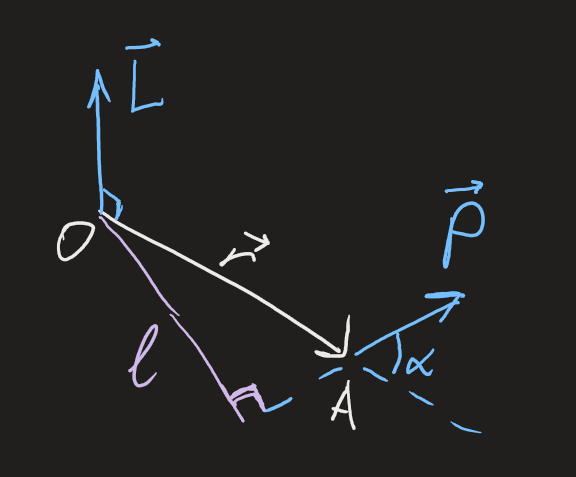
\includegraphics[width=0.3\textwidth]{physics1/images/physics1_2024_10_07_4}
            \end{wrapfigure}

            \item Момент импульса $L$

            Аналогично моменту силы можем определить момент импульса:

            $\vec{L} = [\vec{r} \vec{p}]$
            
            $L = r \cdot p \cdot \sin\alpha = p \cdot l$
            
            $[L] = \text{кг} \frac{\text{м}^2}{\text{с}} = \text{Н} \cdot \text{с} \cdot \text{м}$

            \item Уравнение моментов

            $\frac{d\vec{L}}{dt} = [\frac{d\vec{r}}{dt}\vec{p}] + [\vec{r} \frac{d\vec{p}}{dt}] = \cancelto{0}{[\vec{v} \vec{p}]} + [\vec{r} \vec{F}] = \vec{M}$ \hfill $\cancelto{0}{[\vec{v} \vec{p}]} \Longleftarrow \vec{v} \uparrow\uparrow \vec{p}$

            \fbox{$\frac{d\vec{L}}{dt} = \vec{M}$}
        \end{minipage}

        \smallvspace

        $\frac{d\vec{p}}{dt} = \vec{F} \quad \Longrightarrow \quad \vec{F}_\text{внешн} = 0 \Longrightarrow \vec{p} = const$ - закон сохранения импульса

        \smallvspace

        \begin{minipage}{\textwidth}
            \begin{wrapfigure}{r}{0pt}
                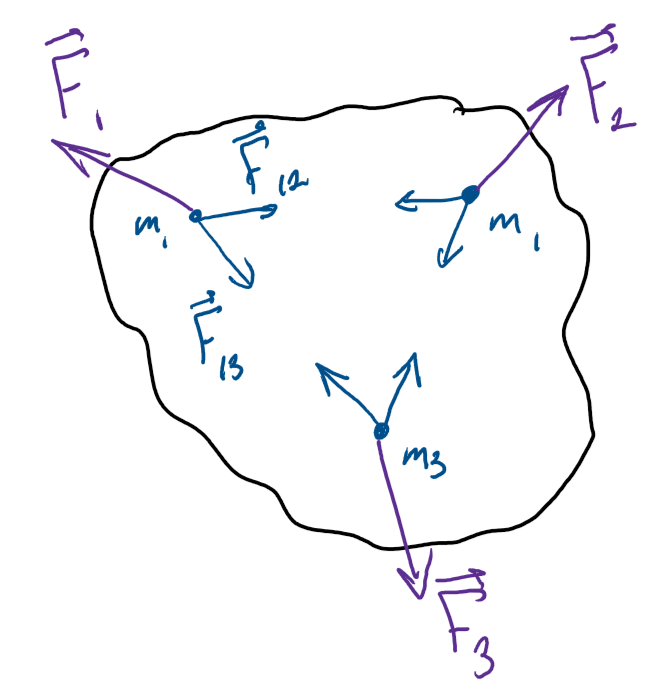
\includegraphics[width=0.3\textwidth]{physics1/images/physics1_2024_10_07_5}
            \end{wrapfigure}

            \item Закон сохранения момента импульса

            Пусть дана система материальных точек. На них действуют силы, которые мы можен разделить на внутренние и внешние

            В замкнутой системе внешние силы сведены к 0:

            $\frac{d\vec{L}}{dt} = \vec{M} = \vec{M}_{\text{внешн}} + \cancelto{0}{\vec{M}_{\text{внутр}}}$

            Поэтому:

            $\vec{M}_\text{внешн} = 0 \Longrightarrow \vec{L} = const$ - закон сохранения момента импульса

            \item Основное уравнение динамики вращательного движения

            $L_i = m_i v_i \cdot r_i = m_i \omega \cdot r_i^2 = \omega m_i r_i^2$
        \end{minipage}

        \smallvspace

        \begin{minipage}{\textwidth}
            \begin{wrapfigure}{r}{0pt}
                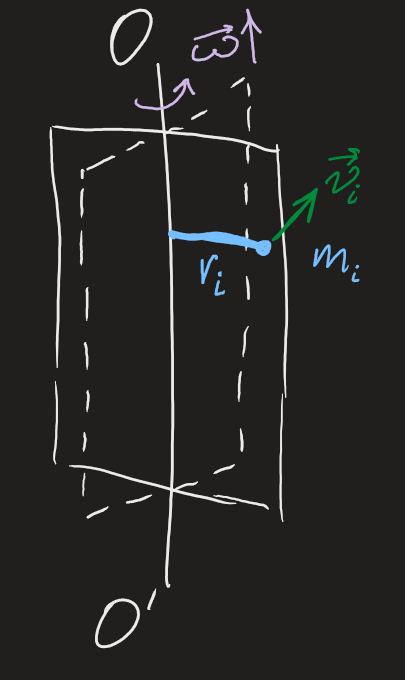
\includegraphics[width=0.2\textwidth]{physics1/images/physics1_2024_10_07_6}
            \end{wrapfigure}


            $L = \sum L_i = \omega \sum m_i r_i^2$

            $\vec{p} = m \vec{v} \qquad L_z = I \omega_z$

            $I = \sum m_i r_i^2$ - момент инерции системы материальных точек, $[I] = \text{с} \cdot \text{м}^2$

            В интегральной форме: $I = \int r^2 dm$

            Здесь же выделим различное распределение массы
        \end{minipage}

        \smallvspace
        
        \begin{enumerate}[label=\alph*) ]
            \item Линейное: $\tau = \frac{dm}{dl} = \frac{m}{l}$

            \item Поверхностное: $\sigma = \frac{m}{s} = \frac{dm}{ds}$

            \item Объемное: $\rho = \frac{m}{V} = \frac{dm}{dV}$
        \end{enumerate}

        $L_z = I \omega_z$

        $\frac{dL_z}{dt} = I \frac{d\omega_z}{dt} = I \beta_z$

        \fbox{$M_z = I \beta_z$} - основное уравнение динамики вращательного движения

        \item Расчет моментов инерции твердых тел

        Рассмотрим моменты инерции для твердых тел разной формы:

        \smallvspace
            
        \begin{enumerate}
            \begin{minipage}{0.95\textwidth}
                \begin{wrapfigure}{r}{0pt}
                    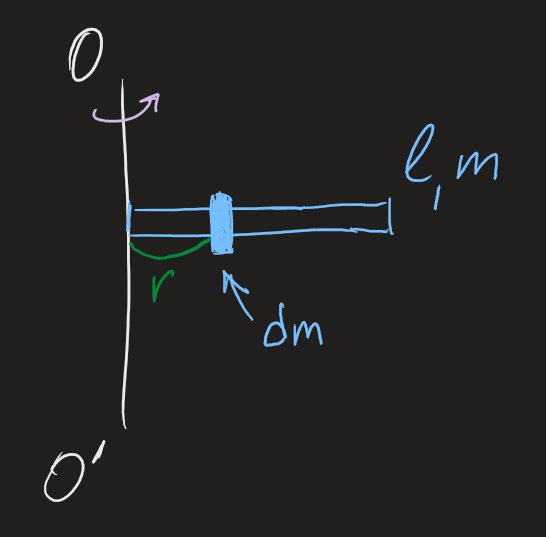
\includegraphics[width=0.2\textwidth]{physics1/images/physics1_2024_10_07_7}
                \end{wrapfigure}


                \item \textbf{Стержень}

                $I = \int r^2 dm$

                $I_{\text{м.т.}} = mr^2$

                $dI = r^2 \dm$

                $I = \sum_{i} d I_i = \int_0^l dI = \int_0^l r^2 dm = \int_0^l r^2 \tau dl = \int_0^l r^2 \tau dr = \tau \frac{r^3}{3} \Big|_0^l = \tau \frac{l^3}{3} = \frac{ml^2}{3}$

                \fbox{$I_\text{стерж} = \frac{ml^2}{3}$}

            \end{minipage}

            \begin{minipage}{0.95\textwidth}
                \begin{wrapfigure}{r}{0pt}
                    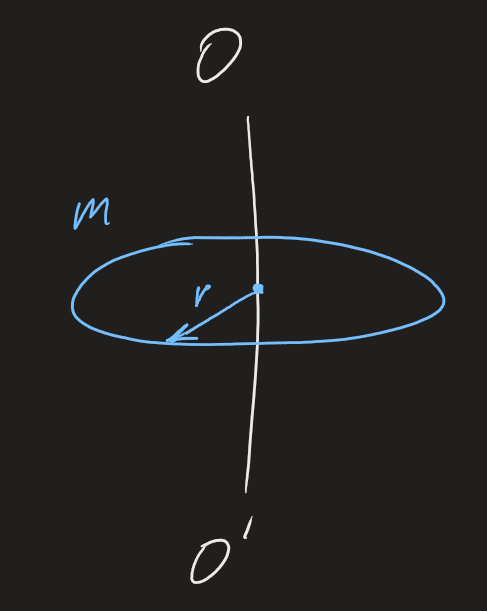
\includegraphics[width=0.2\textwidth]{physics1/images/physics1_2024_10_07_8}
                \end{wrapfigure}

                \item \textbf{Кольцо}

                Для кольца тривиально: \fbox{$I_\text{кольц} = r^2 m$}
                
                \item \textbf{Диск}

                Разбиваем диск на кольца с радиусом $r$ толщиной $dr$

                $dI = dm r^2 = \sigma ds r^2 = \sigma 2\pi r dr r^2 = \sigma ds r^2$

                $I = \int \sigma 2\pi r^3 dr = \sigma 2\pi \frac{R^4}{4} = \frac{mR^2}{2}$

                \fbox{$I_\text{диск} = \frac{mR^2}{2}$}

            \end{minipage}

            \begin{minipage}{0.95\textwidth}
                \begin{wrapfigure}{r}{0pt}
                    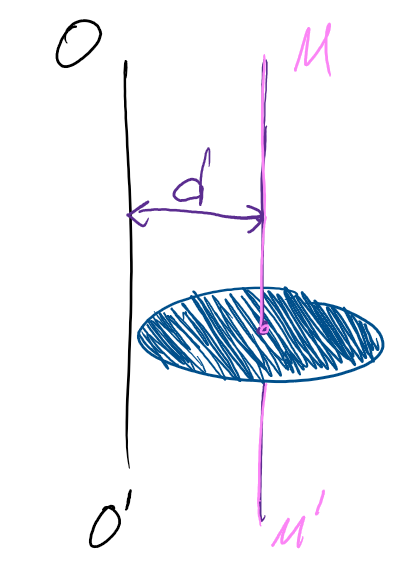
\includegraphics[width=0.2\textwidth]{physics1/images/physics1_2024_10_07_9}
                \end{wrapfigure}

                \item \textbf{Теорема Штейнера}

                Теорема Штейнера гласит, что момент инерции тела для неподвижной оси равен сумме момента инерции для оси тела, проходящей через центр масс и параллельной исходной и произведению квадрата расстояния и массы

                $I = I_0 + md^2$

                Пример: кольцо вращается вокруг оси, расположенной на торце кольца, зная момент импульса в центральной оси кольца 
                и расстояние между осями, можем узнать момент импульса для кольца

            \end{minipage}
        \end{enumerate}


    \end{enumerate}
% end physics1_2024_10_07.tex

% begin physics1_2024_10_14.tex

    \section{6. Гироскоп. Механическая работа.}

    Повторим то, что было на прошлой лекции. Рассмотрим два типа движения:

    \mediumvspace

    \begin{multicols}{2}
        \begin{tcolorbox}[title=Поступательное движение]
            $d\vec{r}; x, y, z$

            $\vec{v} = \frac{d\vec{r}}{dt}$

            $\vec{a}_\tau = \frac{d\vec{v}}{dt}$

            $m$

            $\vec{p} = m\vec{v}$

            $\vec{p} = const$ при $\vec{F}_\text{вн.} = 0$ (ЗСИ)

            $\vec{F} = m\vec{a}$

            $\vec{F} = \frac{d\vec{p}}{dt}$
        \end{tcolorbox}
        
        \begin{tcolorbox}[title=Вращательное движение]
            $d\vec{\varphi}$

            $\vec{\omega} = \frac{d\vec{\varphi}}{dt}$

            $\vec{\beta} = \frac{d\vec{\omega}}{dt}$

            $I \qquad I_{\text{м.т.}} = mr^2, \hfill I = \int r^2 dm$

            $\vec{L} = I \vec{\omega} \hfill \vec{L} = [\vec{r}\vec{p}]$

            $\vec{L} = const$ при $\vec{M}_\text{вн} = 0$ (ЗСМИ)

            $M_z = I\beta_z$

            $\vec{M} = \frac{d\vec{L}}{dt} \hfil = [\vec{r}\vec{F}]$
        \end{tcolorbox}
    \end{multicols}

    \smallvspace
    
    \begin{minipage}{\textwidth}
        \begin{wrapfigure}{r}{0pt}
            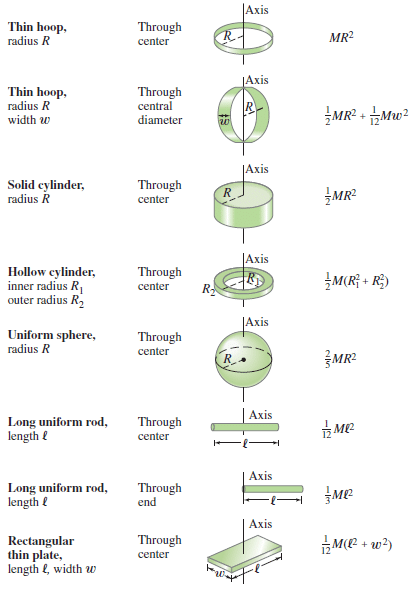
\includegraphics[width=6cm]{physics1/images/physics1_2024_10_14_1}
        \end{wrapfigure}

        Теорема Штейнера: момент инерции $I$ тела относительно произвольной неподвижной оси равен сумме момента инерции этого тела 
        $I_0$ относительно параллельной ей оси, проходящей через центр масс тела, и произведения массы тела $m$ на квадрат расстояния 
        $d$ между осями:

        \[I = I_0 + md^2\]

        Также мы рассмотрели моменты инерции для разных тел

        \subsection{Гироскоп}

        Рассмотрим вращающийся волчок: вращаясь, он постепенно теряет энергию из-за трения и сопротивления воздуха, из-за чего
        его вращение замедляется, и его ось начинает вращаться по другой оси. 
    \end{minipage}
        
    \begin{minipage}{\textwidth}
        \begin{wrapfigure}{r}{0pt}
            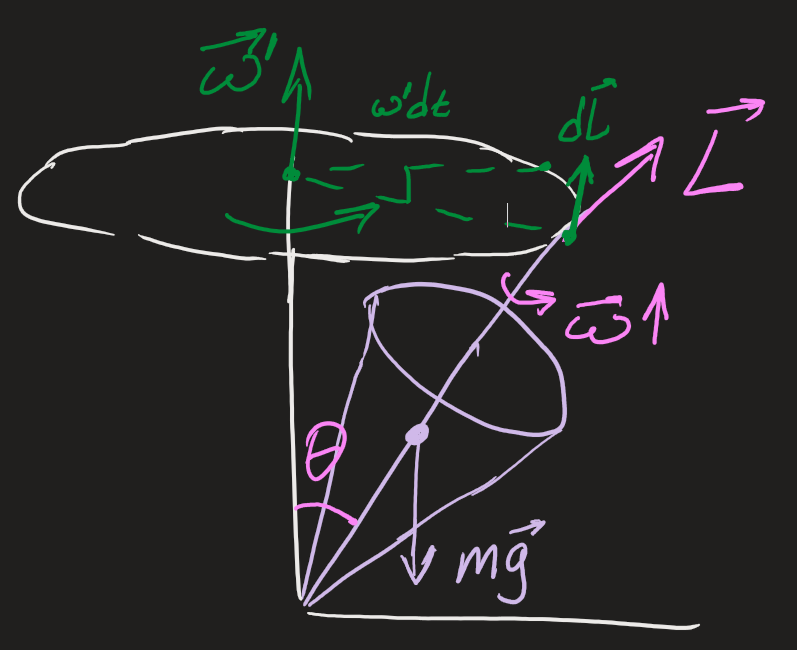
\includegraphics[width=6cm]{physics1/images/physics1_2024_10_14_2}
        \end{wrapfigure}
        
        Обозначим за $\vec{L}_\omega$ момент инерции 
        волчка и за $\vec{L}^\prime$ момент инерции оси. Тогда:
        
        $\vec{L} = \vec{L}_\omega + \vec{L}^\prime$

        $\vec{L}_\omega = I \vec{\omega}$

        Заметим, что в опыте скорость вращения волчка намного больше скорости вращения оси $\omega \gg \omega^\prime$

        Из этого $d\vec{L} = L \sin\theta \cdot \omega^\prime dt$

    \end{minipage}
    
    \smallvspace

    Или в векторной форме:

    $d\vec{L} = [\vec{\omega}\vec{L}]dt$

    $\vec{M} = [\vec{\omega}\vec{L}]$

    Также заметим, что $L_\omega \gg L^\prime$

    Способность сохранять положение вращающегося волчка используется в таком приборе, как гироскоп. 
    Гироскоп применяется для определения положения аппарата (например, самолет, космического корабля) в авионике.



    \subsection{Механическая работа}

    $d\vec{r}$ - элементарное перемещение, в пределах которого сила $\vec{F}$ постоянна

    $Fs$ - проекция силы на направление перемещения

    $d\vec{r} = ds$

    Элементарная работа силы $\vec{F}$ на перемещении $d\vec{r}$

    $dA = \vec{F} d\vec{r} = F\cdot ds \cos \alpha = F_s ds$

    $A = \sum dA = \int dA$

    $A = \int_1^2 \vec{F}d\vec{r} = \int_1^2 F_s ds$

    Допустим на тело действует несколько сил:

    $\vec{F} = \vec{F}_1 + \vec{F}_2 + \dots$

    $A = \int_1^2 \vec{F}d\vec{r} = \int_1^2 (\vec{F}_1 + \vec{F}_2 + \dots) d\vec{r}$

    Мощность - скалярная величина, равная работе силы, совершаемой за единицу времени. Характеризует скорость, с которой совершается работа

    $N = \frac{dA}{dt} = \frac{\vec{F}d\vec{r}}{dt} = \vec{F}\vec{v}$

    $A = \int Ndt$

    Работа силы упругости: $A = \int_{x_1}^{x_2} (-kx)dx = \frac{kx^2_1}{2} - \frac{kx_2^2}{2}$

    Работа силы тяжести: $A = \int_1^2 m\vec{g}d\vec{r} = mgh_1 - mgh_2$

    Работа силы тяготения: $A = \int_{r_1}^{r_2} \frac{Gm_1 m_2}{r^2} dr = - \frac{Gm_1 m_2}{r} \Big|_{r_1}^{r_2} = \frac{Gm_1 m_2}{r_1} - \frac{Gm_1 m_2}{r_2}$

    Силы, чья работа не зависит от траектории пути, будет называть \textit{консервативными} (потенциальными)

    Тогда из этого мы можем вывести потенциальную энергию:

    Потенциальная энергия для силы упругости: $U = \frac{kx^2}{2}$

    Потенциальная энергия для силы тяжести: $U = mgh$

    Потенциальная энергия для силы тяготения: $U = \frac{Gm_1 m_2}{r}$

    В общем виде получаем $A = U_1 - U_2$

    $dA = -dU \qquad \vec{F}d\vec{r} = -dU$

    $\vec{F} = -(\frac{\partial u}{\partial x}\vec{i} + \frac{\partial u}{\partial y}\vec{j} + \frac{\partial u}{\partial z}\vec{k})$

    $\vec{F} = -\mathrm{grad}\, U = -\nabla U$
% end physics1_2024_10_14.tex

% begin physics1_2024_10_21.tex

    \section{7. Закон сохранения энергии.}

    $A = \int \vec{F} d\vec{r} = \int F_s ds \quad F_s = F \cdot \cos\alpha$

    $A_{\text{упр.}} = \frac{kx_1^2}{2} - \frac{kx_2^2}$

    $A = mgh_1 - mgh_2$

    $A = \frac{Gm_1 m_2}{r_1^2} - \frac{Gm_1 m_2}{r_2^2} $

    $A = U_1 - U_2$, \qquad\qquad $U(x, y, z)$ - потенциальная энергия, Дж 

    $dA = -dU$

    $\vec{F}d\vec{r} = -dU$

    $d\vec{r}$ по $Ox$

    $F_x dx = -dU$

    $F_x = -\frac{\partial U}{\partial x}$

    Аналогично для других осей: $F_y = -\frac{\partial U}{\partial y}; \qquad F_z = -\frac{\partial U}{\partial z}$

    $\vec{F} = F_x \vec{i} + F_y \vec{j} + F_z \vec{k}$

    $\vec{F} = -\left(\frac{\partial u}{\partial x}\vec{i} + \frac{\partial u}{\partial y}\vec{j} + \frac{\partial u}{\partial z}\vec{k}\right) = 
    -\mathrm{grad}U$

    $\vec{F}(x, y, z) \longrightarrow U(x, y, z)$

    Например, в электростатике напряженность поля $\vec{E} = -\nabla \varphi$ - это градиент потенциал

    Кинетическая энергия
    
    $A = \int \vec{F}d\vec{r} = \int m \vec{a} d\vec{r} = \int m \frac{d\vec{v}}{dt} d\vec{r} = \int_{v_1}^{v_2} m \vec{v} d\vec{v} = \frac{mv_2^2}{2} - \frac{mv_1^2}{2}$

    $A = U_1 - U_2$

    Энергия вращательного движения

    $E_\text{кин} = \frac{mv^2}{2} = \frac{m\omega^2 r^2}{2} = \frac{I\omega^2}{2}$

    Работа при вращательном движении

    $dA = \vec{F}_i d\vec{r}_i = F_{r_i} dr = F_{r_i} r_i d\varphi_i = M_i d\varphi_i$

    $A = \int \vec{M}d\vec{\varphi} = \int \vec{F}d\vec{r}$

    Механическая энергия - скалярная физическая величина, характеризующая способность тел совершать работу

    $E_\text{мех} = E_k + U$ - сумма кинетической и потенциальной энергий

    Кинетическая энергия - функция состояния движения системы: $E_k = \frac{mv^2}{2} = \frac{p^2}{2m}$

    Потенциальная энергия - функция состояния системы $U(x, y, z)$

    Работа всех сил:

    $A_{12} + A_\text{внешн} = E_{\text{к}2} - E_{\text{к}1}$

    $A_\text{внешн} = (E_{\text{к}2} + U_2) - (E_{\text{к}1} + U_1) = E_\text{мех2} - E_\text{мех1} = \Delta E$

    Если работа внешних сил равна нулю, то $\Delta E = 0 \Longleftrightarrow E_\text{мех} = E_\text{к} + U = const$ 
    
    Закон сохранения энергии: полная механическая энергия замкнутой системы тел, между которым действуют только консервативные силы остается постоянной

    Если в системе действуют неконсервативные силы, из-за которых механическая энергия системы уменьшается, то такие силы называют диссипативными. 
    При этом общий ЗСЭ выполняется: потерянная энергия переходит в другие виды, например, тепловую.

    \textit{Энергия никогда не создается и не уничтожается - она переходит из одной формы в другой.}

    \mediumvspace

    \underline{Задача}: полнотелый шарик радиуса $r$ катится со склона с высоты $H$, на конце склона есть мертвая петля радиуса $R$.
    Какая изначальная высота склона $H$ должна быть у шара, чтобы он смог прокатиться по мертвой петле.

    \smallvspace

    \begin{minipage}{\textwidth}
        \begin{wrapfigure}{r}{0pt}
            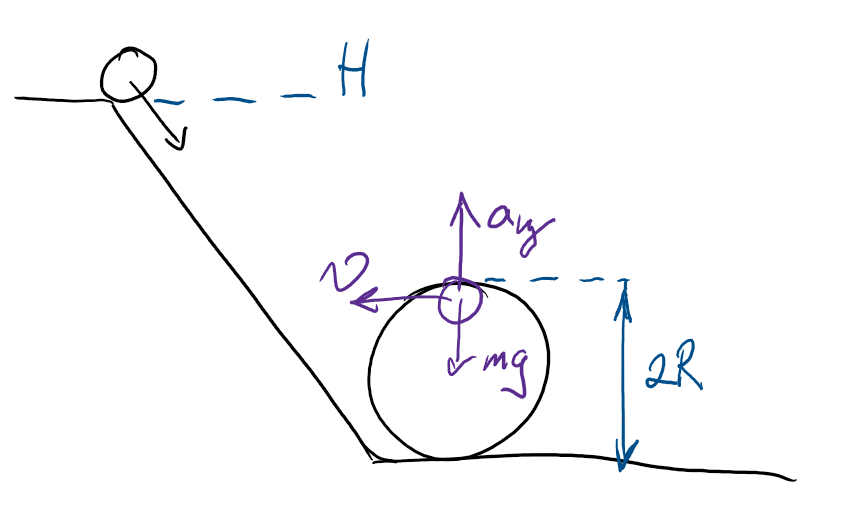
\includegraphics[height=5cm]{physics1/images/physics1_2024_10_21_1}
        \end{wrapfigure}
        
        Условие прохождения шара по мертвой петле: 
        
        $mg = a_{\text{ц}} = \frac{mv^2}{R} \quad \Longrightarrow \quad v = \sqrt{gR}$

        Кинетическая энергия в верхней точке петли: 
        
        $E_\text{к} = \frac{mv^2}{2} + \frac{I\omega^2}{2}$

        Шар катится без скольжения, значит имеет место быть вращательное движение, момент инерции для полнотелого шара $I = \frac{2}{3}mr^2$

        Получаем $mgH = 2mgR + \frac{mv^2}{2} + \frac{I\omega^2}{2} = 2mgR + \frac{mv^2}{2} + \frac{1}{3}mr^2 \cdot \frac{v^2}{r^2} = 
        2mgR + \frac{5}{6}mv^2$

        $h = 2R + \frac{5v^2}{6g} = 2R + \frac{5}{6}R = \frac{17}{6}R$
    \end{minipage}
% end physics1_2024_10_21.tex

% begin physics1_2024_10_28.tex

    \section{8. Тепловые явления.}

    Тепловые явления в физике изучают 2 раздела: молекулярная кинетическая теория (МКТ) и термодинамика. 
    МКТ обычно изучает макроскопические системы, используя статистику, а термодинамика описывает
    макросистемы, исходя из глобальных параметров

    Здесь же исследователи выделили основные положения МКТ: все тела состоят из очень большого числа частиц, 
    и эти частицы постоянно находятся в хаотичном, беспорядочном движении - броуновском движении

    Возьмем поршень и посчитаем давление на него - силу на единицу площади:

    $p = \frac{F}{S} \Longrightarrow F = p \cdot S$

    Работа силы давления:

    $dA = \vec{F} \cdot d\vec{s} = p \cdot S \cdot dx$

    $A = \int pS dx = \int p dV$

    Или знакомая со школы формула $A = p\Delta V$ при $p = const$ (изобарный процесс)

    Внутренняя энергия молекул идеального газа $U = \frac{i}{2} \nu R T$

    $i$ - степень свободы

    $\nu$ - количество вещества (в молях)

    $R = 8.31\ \frac{\text{Дж}}{\text{моль} \cdot \text{К}}$ - универсальная газовая постоянная

    $T$ - температура ($T = t^\circ C + 273.15$ К)

    Или для одной молекулы $U = \frac{i}{2} kT$

    $k = 1.38 \cdot 10^{-23}\ \frac{\text{Дж}}{\text{К}}$ - постоянная Больцмана

    На каждую степень свободы молекулы приходится $\frac{1}{2}kT$

    У инертных газов степень свободы - 3

    У двухатомных газов степень свободы - 5 (еще 2 вращательных)

    У молекул газов, состоящих из более 2 атомов, степень свободы - 6

    $Q = A + \Delta U$ - количество теплоты, которое получает газ, преобразовывается в работу и изменение внутренней энергии

    Закон сохранения тепловой энергии - \textit{первое начало термодинамики}

    Равновесное состояние - состояние системы, при котором нет направленного движения вещества или энергии 
    между ее составляющими или между системой и окружающей средой. 
    Обратимым может быть только равновесный процесс

    Второе начало термодинамики гласит: энтропия либо остаётся неизменной, либо возрастает в неравновесных процессах, 
    достигая максимума при установлении термодинамического равновесия

    Элементарное приращение энтропии: $dS = \frac{dQ}{T}$

    $\Delta S = \int_1^2 \frac{dQ}{T}$

    Для обратимых процессов $\Delta S = 0 \Longrightarrow S = \mathrm{const}$

    Для необратимых $\Delta S > 0 \Longrightarrow S \uparrow$

    
% end physics1_2024_10_28.tex

% begin physics1_2024_11_15.tex

    \section{9. Электрическое поле в вакууме}

    \subsection{Электромагнитное взаимодействие}

    Электромагнитное взаимодействие - одно из четырёх фундаментальных взаимодействий, 
    оно существует между частицами, обладающими электрическим зарядом

    Электрон переводится с древнегреческого как янтарь - греки заметили, что натертый мехом янтарь притягивает вещи

    С тех пор человек обозначил заряд положительным, если в теле образовался его избыток, и отрицательным при его дефиците.

    У. Гильберт предложил первый электроскоп: два лепестка фольги в банке, соединенные с металлическим шариком,
    при касании заряженного предметом шарика лепестки расходятся

    В 1861 году Максвелл вывел уравнения Максвелла, который стали основой классической электродинамикой:

    \begin{tcolorbox}[title=Уравнения Максвелла, colframe=green!25, colback=green!10, coltitle=black]
        \begin{gather*}
            \oint_l \vec{E} d\vec{l} = -\int_S \frac{\partial \vec{B}}{\partial t} d\vec{S}\\
            \oint_l \vec{H} d\vec{l} = I_{\text{полн}} = \int_S (\vec{j} - \frac{\partial \vec{D}}{\partial t}) d\vec{S}\\
            \oint \vec{D} d\vec{S} = \int_V \rho dV\\
            \int_S \vec{B} d\vec{S} = 0
        \end{gather*}
    \end{tcolorbox}

    \underline{Смысл уравнений}:

    1 уравнение: изменение магнитной индукции порождает вихревое электрическое поле - закон электромагнитной индукции Фарадея

    2 уравнение: переменное электрическое поле $D$ и электрический ток $\vec{j}$ будут вызывать магнитное поле - теорема о циркуляции магнитного поля

    3 уравнение: электрический заряд порождает электрическую индукции - закон Гаусса

    4 уравнение: поток магнитной индукции через замкнутую поверхность равен нулю - закон Гаусса для магнитного поля

    Эти уравнения можно переписать в дифференциальной форме:

    \begin{tcolorbox}[colframe=green!25, colback=green!10]
        \begin{gather*}
            \mathrm{rot} \vec{E} = -\frac{\partial \vec{B}}{\partial t}\\
            \mathrm{rot} \vec{H} = \vec{j} + \frac{\partial \vec{D}}{\partial t}\\
            \mathrm{div} \vec{D} = \rho\\
            \mathrm{div} \vec{B} = 0
        \end{gather*}
    \end{tcolorbox}

    Второй уравнение можно представить так: $\vec{j} = \sigma \vec{E}$ - 
    плотность тока равна проводимости среды на напряженность поля (закон Ома)

    \textbf{Заряд} - характеристика вещества, показывающая, может ли тело участвовать в электромагнитом взаимодействии

    Милликен показал, что $\overline{e} = -1.6 \cdot 10^{-19}$ Кл 

    Позже были найдены заряд электрона $|p| = -1.6 \cdot 10^{-19}$ Кл, массы электрона $m_{\overline{e}} = 9.1 \cdot 10^{-31}$ кг и протона $m_p = 1836 \cdot m_{\overline{e}} = 1.67 \cdot 10^{-27}$ кг

    Отрицательно заряженное тело - тело, где электронов больше, чем протонов; положительное тело - тело, где электронов меньше, чем протонов

    Если тело не заряжено, то его суммарный заряд равен нулю

    \smallvspace

    \begin{minipage}{\textwidth}
        \begin{wrapfigure}{r}{0pt}
            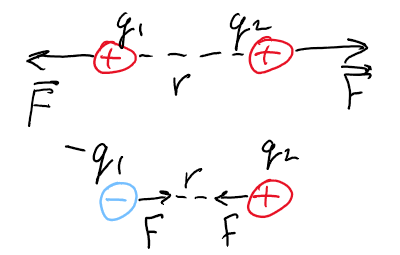
\includegraphics[width=5cm]{physics1/images/physics1_2024_11_15_3}
        \end{wrapfigure}

        \textbf{Точечный заряд} - заряженное тело, размерами которого можно пренебречь по сравнению с расстоянием до других заряженных тел

        Путем бесчисленного количества опытов Кулон установил, что $|F| \sim \frac{1}{r^2} \sim q_1 \sim q_2$

        В итоге появилась сила Кулона в вакууме: 
        $\vec{F} = \frac{k|q_1| |q_2|}{r^3} \vec{r}$

        $k = \frac{1}{4\pi \varepsilon_0} = 9 \cdot 10^9 \ \frac{\text{Н} \cdot \text{м}^2}{\text{Кл}^2}$

        $\varepsilon_0 = 8.85 \cdot 10^{-12} \ \frac{\text{Ф}}{\text{м}}$
    \end{minipage}
    

    \textbf{Электрическое (электромагнитное) поле} - определенная форма материи,
    через которую осуществляются электромагнитные взаимодействия. Любое заряженное тело, помещенное в какую-либо точку поля
    оказывается под воздействием силы.

    \textbf{Электростатическое поле} - поле неподвижных зарядов

    \textbf{Пробный заряд} - точечный положительный заряд, который не искажает исследуемое поле, то есть не вызывает в нем перераспределения зарядов

    Выделяют 2 характеристики поля:

    \begin{itemize}
        \item Напряженность (силовая)

        \item Потенциал (энергетическая)
    \end{itemize}

    \textbf{Напряженность электрического поля} - векторная величина, численно равная силе, действующей на единичный положительный заряд, помещенный в данную точку поля.
    Вектор напряженности совпадает по направлению с силой, действующей на \enquote{+} заряд

    $\vec{E} = \frac{\vec{F}}{q}$ \hfill $[E] = \frac{\text{В}}{\text{м}}$

    $\vec{E} = \frac{k|q|}{r^3}\vec{r}$ - напряженность поля точечного заряда

    \textbf{Линии напряженности} - линии, касательные к которым в каждой точке поля направлены также, как и вектор напряженности. 
    Линии напряженности начинаются на положительных зарядах, заканчиваются на отрицательных зарядах. Линии не пересекаются, не замкнуты. 
    Густота линий напряженности пропорциональна модулю вектора напряженности электрического поля

    Диполь - система из равных по модулю, но разных по знаку точечных зарядов

    \begin{multicols}{3}
        \begin{center}
            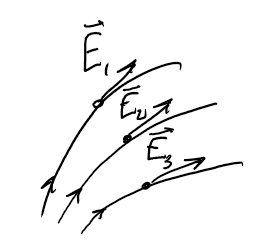
\includegraphics[width=5cm]{physics1/images/physics1_2024_11_15_4}
        \end{center}

        \begin{center}
            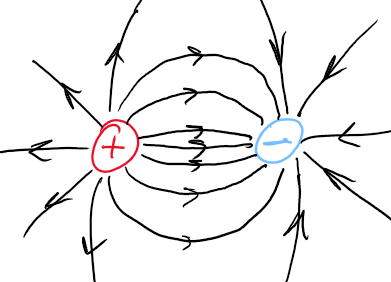
\includegraphics[width=5cm]{physics1/images/physics1_2024_11_15_5}
        \end{center}

        \begin{center}
            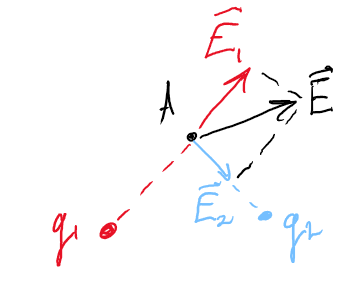
\includegraphics[width=5cm]{physics1/images/physics1_2024_11_15_6}
        \end{center}
    \end{multicols}

    \textbf{Принцип суперпозиции}: напряженность поля системы зарядов равна векторной сумме напряженностей полей, которое создает каждый из этих зарядов в отдельности

    \[\vec{E} = \vec{E}_1 + \vec{E}_2 + \dots + \vec{E}_n\]

    \textbf{Однородное поле} - поле, в каждой точке которого напряженность одинакова по модулю и направлению, например, поле конденсатора

    \textbf{Линейная плотность заряда} (однородное распределение заряда): $\tau = \frac{dq}{dl} = \frac{q}{l} \hfill [\tau] = \frac{\text{Кл}}{\text{м}}$

    \textbf{Поверхностная плотность заряда} $\sigma = \frac{dq}{dS} = \frac{q}{S} \hfill [\sigma] = \frac{\text{Кл}}{\text{м}^2}$

    \textbf{Объемная плотность заряда} $\rho = \frac{dq}{dV} = \frac{q}{V} \hfill [\rho] = \frac{\text{Кл}}{\text{м}^3}$


    \begin{minipage}{\textwidth}
        \textbf{Поле на оси тонкого равномерно-заряженного кольца}:
        
        \begin{wrapfigure}{r}{0pt}
            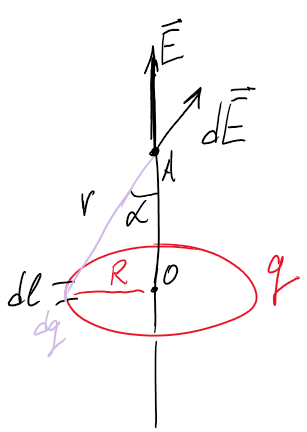
\includegraphics[width=5cm]{physics1/images/physics1_2024_11_15_1}
        \end{wrapfigure}

        Заряд $q$ равномерно распределен по тонкому кольцу радиусом $R$. Найти напряженность,
        создаваемую кольцом как функцию расстояния $z$ от его центра

        $E = \int_l dE = \int_l k \frac{dq}{z^2 + R^2}$

        $dE z = dE \cos\alpha$

        $E = \sum dE \cdot z = \int dE \cdot z = \int k \frac{dq}{r^2} \cdot z$

        $E = \int \frac{k dq}{r^2} \cos\alpha = \frac{k \cos\alpha}{r^2} \int dq = \frac{k q \cos \alpha}{r^2}$

        $\cos \alpha = \frac{z}{r}$

        $r = \sqrt{R^2 + z^2}$

        $E = \frac{kqz}{(R^2 + z^2)^{\frac{3}{2}}}$
        
    \end{minipage}

    Заметим, что в центре кольца напряженность нулевая

    При слишком больших $z$ получаем формулу напряженность для точечного заряда - размерами кольца можно пренебречь

    \mediumvspace

    

    \begin{minipage}{\textwidth}
        \textbf{Поле равномерно-заряженной прямой нити}:
        
        \begin{wrapfigure}{r}{0pt}
            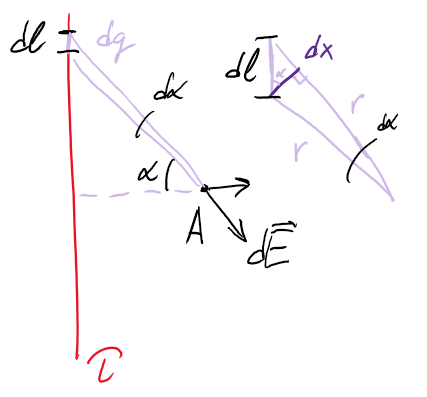
\includegraphics[width=7cm]{physics1/images/physics1_2024_11_15_2}
        \end{wrapfigure}

        Бесконечная прямая нить равномерно заряжена с линейной плотностью $\tau$.
        Найти напряженность, создаваемую нитью на расстоянии $a$ от ее центра 
    
        В силу симметрии напряженность будет направлена вправо
    
        $dE_x = dE \cos\alpha = \frac{kdq}{r^2} \cos\alpha$
    
        $dq = \tau dl = \left[dl = \frac{dx}{\cos\alpha} = \frac{rd\alpha}{\cos\alpha}\right] = \tau \frac{rd\alpha}{\cos\alpha}$
    
        $dE_x = \frac{k\tau rd\alpha}{r^2 \cos\alpha} \cos\alpha = \frac{k\tau d\alpha}{r} = \left[r = \frac{a}{\cos\alpha}\right] = 
        \frac{k\tau}{a}\cos\alpha d\alpha$
    
        $E = \frac{k\tau}{a} \int_{-\frac{\pi}{2}}^{\frac{\pi}{2}} \cos\alpha d\alpha = \frac{2k\tau}{a}$
    
        $E = \frac{2k\tau}{a}$
    \end{minipage}

   
    \subsection{Теорема Гаусса-Остроградского}

    \textit{Подробнее о теореме можно прочитать в \href{https://pelmesh619.github.io/itmo_conspects/conspects/calculus/calculus_superconspect.pdf}{конспекте математического анализа}}

    \mediumvspace

    \begin{minipage}{\textwidth}
        \begin{wrapfigure}{r}{0pt}
            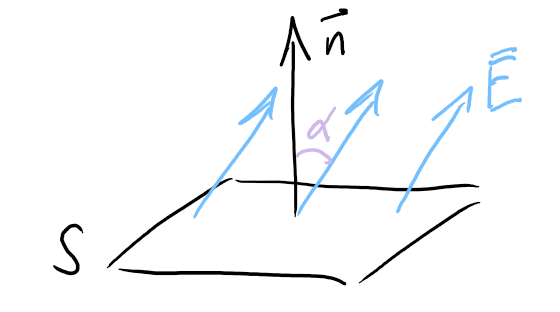
\includegraphics[width=5cm]{physics1/images/physics1_2024_11_15_7}
        \end{wrapfigure}

        Поток вектора напряженности электрического поля
    
        Поток $d\Phi = \vec{E}\cdot d\vec{S} = E_n dS = E \cdot dS \cdot \cos\alpha$

        Поток пропорционален числу линий напряженности электрического поля, пронизывающих площадку $dS$

        $[\Phi] = \frac{\text{В}}{\text{м}} \cdot \text{м}^2 = \text{В} \cdot \text{м}$

    \end{minipage}

    \begin{minipage}{\textwidth}
        \begin{wrapfigure}{r}{0pt}
            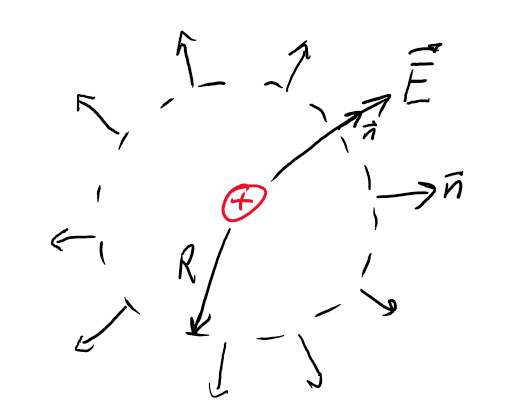
\includegraphics[width=7cm]{physics1/images/physics1_2024_11_15_8}
        \end{wrapfigure}
    
        Через произвольную поверхность $\Phi = \int_S d\Phi = \int \vec{E} d\vec{S}$. Отсюда $\Phi = E \cdot S \cdot \cos\alpha$

        Заряд $q$ в центре замкнутой сферической поверхности

        $\Phi = \oint \vec{E} d\vec{s} \quad \vec{E} \uparrow\uparrow \vec{n}$

        $E = \frac{kq}{r^2} = \mathrm{const}$

        $\Phi = \frac{kq}{r^2} \cdot S = \frac{1}{4\pi \varepsilon_0} \frac{q}{r^2} \cdot 4\pi r^2 = \frac{q}{\varepsilon_0}$

        $\oint \vec{E}d\vec{S} = \Phi = \frac{q_{\text{внутр}}}{\varepsilon_0}$ - теорема Гаусса-Остроградского

    \end{minipage}
% end physics1_2024_11_15.tex



\end{document}

